\documentclass[10pt,aspectratio=169,t]{beamer}

% ─── Theme & colors ─────────────────────────────────────────────────────────
\usetheme{metropolis}
\usepackage{appendixnumberbeamer}
\usepackage{booktabs}
\usepackage{verbatim}
\usepackage{amsmath, amssymb}
\usepackage{graphicx}
\usepackage{xcolor}
\usepackage{tikz}
\usepackage{CJKutf8}
\usepackage{dsfont}
\usetikzlibrary{arrows.meta, positioning, shapes.geometric, fit}

\definecolor{spblue}{RGB}{0, 51, 102}
\definecolor{spred}{RGB}{180, 30, 50}
\definecolor{spgray}{RGB}{100, 100, 100}
\setbeamercolor{frametitle}{bg=spblue}
\setbeamercolor{progress bar}{fg=spred}
\setbeamercolor{title separator}{fg=spred}
\usepackage{etoolbox}
\AtBeginEnvironment{frame}{%
  \setlength{\abovedisplayskip}{2pt}
  \setlength{\belowdisplayskip}{2pt}
  \setlength{\abovedisplayshortskip}{1pt}
  \setlength{\belowdisplayshortskip}{1pt}
}

% ─── Title page metadata ────────────────────────────────────────────────────
\title{Rule-Based Monetary Policy in China}
\subtitle{A Counterfactual Analysis Using the Caravello et al.\ (2025) Framework}
\author{Liming Lin}
\institute{Sciences Po Paris \\ \small Supervisor: Paul Bouscasse\\
\small Jury: Paul Bouscasse, Axelle Ferrière}
\date{April 2025 — \textit{Work in Progress}}
\begin{document}

% ─── Title slide ────────────────────────────────────────────────────────────
\maketitle

% ═══════════════════════════════════════════════════════════════════════════
% SLIDE 1 — MOTIVATION & RESEARCH QUESTION
% ═══════════════════════════════════════════════════════════════════════════
\begin{frame}{Motivation}

\textbf{The puzzle.} Since 2023, Chinese CPI inflation has hovered near zero,
persistently undershooting the official targets set in the annual Government
Work Report (GWR).


\begin{itemize}
  \item GWR CPI targets 2023--2025: \textbf{3\%, 3\%, 2\%}
  \item Realized CPI YoY 2023--2025: roughly \textbf{0\%}
  \item Xi's speech at the 2024 Central Economic Work Conference first
        introduced the phrase ``a reasonable rebound in the price level''
        (\begin{CJK}{UTF8}{gbsn}物价合理回升\end{CJK}); the 2025 CEWC
        explicitly tied this objective to the conduct of monetary policy.
\end{itemize}

\textbf{The question.} What would have happened to the Chinese economy if
the PBoC had strictly followed some form of rule-based policy during this
period?

\textbf{Why it matters.}
\begin{itemize}
  \item Quantifies the policy gap: how far was actual policy from
        target-consistent policy?
  \item Tests whether conventional interest rate policy is even capable
        of closing the inflation gap, given China's transmission mechanism.
\end{itemize}

\end{frame}

% ═══════════════════════════════════════════════════════════════════════════
% SLIDE 2 — METHODOLOGY ROADMAP
% ═══════════════════════════════════════════════════════════════════════════
\begin{frame}{Methodology Roadmap}

Following Caravello, McKay \& Wolf (2025), the empirics-only counterfactual
requires \textbf{four building blocks}:

\vspace{0.6em}
\begin{center}
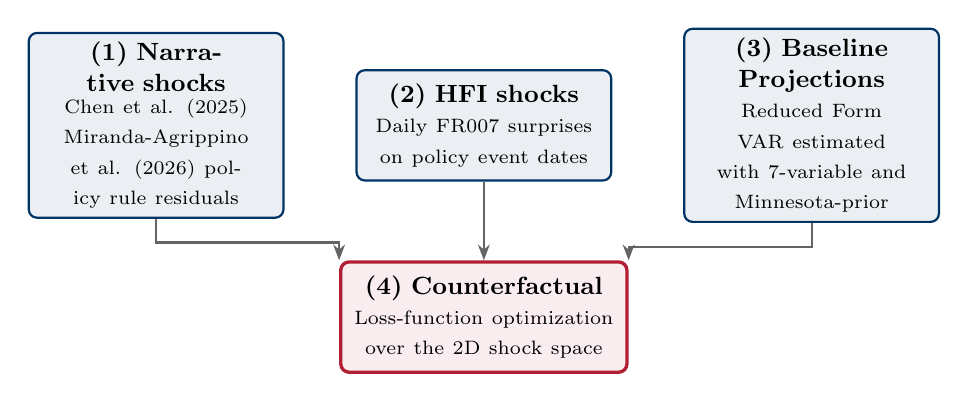
\begin{tikzpicture}[
    node distance=0.7cm and 0.9cm,
    box/.style={
        rectangle, rounded corners=3pt, draw=spblue, thick,
        fill=spblue!8, text width=3.0cm, align=center,
        minimum height=1.4cm, font=\small
    },
    final/.style={
        rectangle, rounded corners=3pt, draw=spred, very thick,
        fill=spred!8, text width=3.4cm, align=center,
        minimum height=1.4cm, font=\small
    },
    arr/.style={-{Stealth[length=2mm]}, thick, spgray}
]

\node[box] (rr) {\textbf{(1) Narrative shocks}\\ \scriptsize Chen et al. (2025) \\ Miranda-Agrippino et al. (2026) policy rule residuals};
\node[box, right=of rr] (hfi) {\textbf{(2) HFI shocks}\\ \scriptsize Daily FR007 surprises on policy event dates};
\node[box, right=of hfi] (ltp) {\textbf{(3) Baseline Projections}\\ \scriptsize Reduced Form VAR estimated with 7-variable and Minnesota-prior};

\node[final, below=1.0cm of hfi] (cf) {\textbf{(4) Counterfactual}\\ \scriptsize Loss-function optimization over the 2D shock space};

\draw[arr] (rr.south) -- ++(0,-0.3) -| (cf.north west);
\draw[arr] (hfi) -- (cf);
\draw[arr] (ltp.south) -- ++(0,-0.3) -| (cf.north east);

\end{tikzpicture}
\end{center}
\end{frame}
% SLIDE 3 — METHODOLOGY ROADMAP EXPLANATION
\begin{frame}{Methodology Roadmap Explanation}
\vspace{0.4em}
\begin{itemize}\itemsep0.2em
  \item Blocks (1) and (2) provide \textbf{two distinct empirical IRFs} of the
        Chinese economy to monetary policy shocks --- the policy ``treatments''
        whose linear combinations span the feasible policy space.
  \item Block (3) provides the \textbf{baseline projection} of where the
        economy goes absent any policy intervention.
  \item Block (4) solves for the shock sequence that moves the baseline
        toward alternative paths, subject to a multi-objective
        loss function.
  \item Using Caravello et al. 2025's framework, instead of traditional counterfactuals based on structural models like DSGE, allows us to avoid the strong assumptions about the underlying economic structure, especially given the unique features of the Chinese institutional and economic environment. 
\end{itemize}

\end{frame}

% ═══════════════════════════════════════════════════════════════════════════
% SLIDE 4 — NARRATIVE SHOCKS
% ═══════════════════════════════════════════════════════════════════════════
\begin{frame}{Narrative Shocks: Estimated Policy Rule}
\hypertarget{slide:rr}{}
 
\textbf{Specification.} A monthly policy rule for the 7-day interbank repo
rate (FR007), combining elements from Chen, Xiao
\& Zha (2025) and Miranda-Agrippino, Nenova \& Rey (2026):

{\small
\begin{align*}
\text{FR007}_t \;=\; \alpha
&\;+\; \rho \cdot \text{FR007}_{t-1}
\;+\; \beta_\pi \cdot \text{cpi\_gap}_{t-1} \\
&\;+\; \beta_y^{+} \cdot \text{gap\_pos}_{t-1}
\;+\; \beta_y^{-} \cdot \text{gap\_neg}_{t-1}
\;+\; \beta_e \cdot \text{fx\_gap}_{t-1}
\;+\; \varepsilon_t^{\text{MP}}
\end{align*}
}

\textbf{Variable definitions.}
\begin{itemize}\itemsep0.15em
  \item[$\bullet$] $\text{cpi\_gap}_t = \pi_t - \pi^{*}_t$, where $\pi^*_t$ is
        the annual CPI target from the Government Work Report
  \item[$\bullet$] $\text{gdp\_gap}_t = g_t - g^{*}_t$, where $g_t$ is a proxy to monthly real GDP YoY
        \textcolor{spgray}{\scriptsize(see appendix:
        \hyperlink{app:gdp}{\beamergotobutton{Stock--Watson construction}})}
        and $g^*_t$ is the GWR growth target
  \item[$\bullet$] $\text{gap\_pos}_t$, $\text{gap\_neg}_t$: asymmetric split of the
        GDP gap around a 1pp threshold
        \textcolor{spgray}{\scriptsize(see appendix:
        \hyperlink{app:regime}{\beamergotobutton{regime-switch motivation}})}
  \item[$\bullet$] $\text{fx\_gap}_t$: post-2006 indicator (when fixed exchange rate regime   ended) interaction between the change in the central parity rate and the spot--parity deviation
\end{itemize}
\end{frame}
\begin{frame}{Narrative Shocks: Identification and Rationale}
\hypertarget{slide:rr2}{}
\textbf{Identification.} The residual $\widehat{\varepsilon}^{\text{MP}}_t$
isolates the unsystematic component of FR007 movements --- the narrative
monetary policy shock series.
\textcolor{spgray}{\scriptsize\hyperlink{app:rrfit}{\beamergotobutton{actual vs.\ predicted FR007}}}
 
\vspace{0.2em}
\textbf{Why this hybrid specification?}
\begin{itemize}\itemsep0.1em
  \item[$\circ$] CXZ2025 kept FR007 as the dependent variable but excluded the
        exchange rate; MANR2026 added the foreign exchange term but used the a Composite Monetary Policy Indicator on the left-hand side.
        \textcolor{spgray}{\scriptsize\hyperlink{app:cmpi_fr007}{\beamergotobutton{CMPI vs.\ FR007}}}
  \item[$\circ$] We retain FR007 (the actual market rate that anchors HFI surprises
        downstream) while adopting MANR2026's FX specification and the lag terms of those gap variables, which mechanically make the policy rates forward-looking.
\end{itemize}
The Impulse Responses to the shocks (also the later HFI shocks and baseline projections) are estimated using a Bayesian SVAR approach with a Minnesota-type prior following Giannone, Lenza \& Primiceri (2015), which was adopted by MANR2026 as well:
\textcolor{spgray}{\scriptsize\hyperlink{app:narr_irf}{\beamergotobutton{Narrative Shocks IRFs}}}
 
\end{frame}

% ═══════════════════════════════════════════════════════════════════════════
% SLIDE 5 — HIGH-FREQUENCY SHOCKS
% ═══════════════════════════════════════════════════════════════════════════
\begin{frame}{High-Frequency Shocks: FR007 Surprises on Policy Event Dates}
\hypertarget{slide:hfi}{}

\textbf{Identification strategy.} Following Das \& Song (2022), we identify monetary policy surprises as the daily close-to-close change in the FR007 rate around dates on which the PBoC announces a change to one of its core policy instruments:

\vspace{-1em}
\[
\text{shock}_t = \bigl(\text{FR007}_t-\text{FR007}_{t-1}\bigr)\cdot\mathds{1}\{t\in\mathcal{E}\}
\]
\vspace{-1em}

where $\mathcal{E}$ is the set of policy event dates.

\textbf{Core policy instruments tracked.} Event dates are collected from PBoC by Wind:

\begin{itemize}
  \item[$\bullet$] 7-day reverse repo rate (OMO) --- the primary short-term policy rate post-2016
  \item[$\bullet$] 1-year Medium-term Lending Facility (MLF) --- introduced 2014, principal medium-term policy tool
  \item[$\bullet$] 1-year Loan Prime Rate (LPR) --- replaced benchmark lending rate as the loan pricing anchor in August 2019
  \item[$\bullet$] Reserve Requirement Ratio for large financial institutions (RRR)
  \item[$\bullet$] Benchmark deposit and lending rates (pre-2015 era, before the rate liberalization)
\end{itemize}
\end{frame}

\begin{frame}{High-Frequency Shocks: Identification and Rationale}

\textbf{Rationale.} Only dates on which the PBoC makes changes to either of the policy instruments are considered are recorded. The reason is that the PBoC makes announcements for certain tools like OMO on a regular basis, which cluster in the later years in the sample and do not necessarily reflect a change in the policy stance.

\textbf{Limitations.} Das \& Song actually used the 1-year Interest Rate Swap (IRS) based on FR007 instead of the FR007 itself to better represent the reactions from the financial markets. However, the access to this data and the more detailed one in hourly frequency have not been granted by the authority yet.\\
In addition, the PBoC's announcements also occur on the same day with other events, including the release of macroeconomic data or the announcements by the fiscal authority, which we also want to come back to revisit if data is available.

\textcolor{spgray}{\scriptsize\hyperlink{app:hfi_series}{\beamergotobutton{monthly HFI shock series}}}

\textcolor{spgray}{\scriptsize\hyperlink{app:hfi_irf}{\beamergotobutton{HFI IRFs}}}

\textcolor{spgray}{\scriptsize\hyperlink{app:hfi_compare}{\beamergotobutton{IRF comparison: any vs.\ rate-change only}}}


\end{frame}

% ═══════════════════════════════════════════════════════════════════════════
% SLIDE 6 — REDUCED-FORM BVAR BASELINE (LTP)
% ═══════════════════════════════════════════════════════════════════════════
\begin{frame}{Reduced-Form Long-Term Projection: Bayesian VAR}

\textbf{Specification.} A 7-variable monthly BVAR with $p=6$ lags.
\[
y_t = c + \sum_{\ell=1}^{6} A_\ell\, y_{t-\ell} + \sum_{k=1}^{4} d_k\, D_t^{\text{covid},k} + u_t,
\qquad
u_t \sim \mathcal{N}(0,\Sigma_u)
\]
where $D_t^{\text{covid},k}$ are monthly dummies for Jan--Apr 2020.

\vspace{0.3em}
\textbf{Variables in $y_t$ (BVAR ordering, monthly).}
{\small
\[
y_t = \bigl(g_t,\, \text{IP}_t,\, \pi_t,\, i_t,\, m_t,\, e_t,\, y_t^{US}\bigr)'
\]
$g_t$: real GDP YoY; $\text{IP}_t$: Industrial Value Added YoY; $\pi_t$: CPI YoY; $i_t$: FR007; $m_t$: M2 YoY growth;\\ $e_t$: RMB Real Effective Exchange Rate YoY; $y_t^{US}$: US output gap YoY; \\Variables reflecting the labor market condition were dropped due to quality and availability issues;\\
Other potential variables like consumption, net exports, and fixed asset investments were excluded because they are already captured by the construction of the monthly GDP proxy.
}

\end{frame}
\begin{frame}{Reduced-Form Long-Term Projection }
\hypertarget{slide:ltp2}{}
\vspace{0.3em}
\textbf{Estimation samples.}
\begin{itemize}\itemsep0.1em
      \item Monthly estimation with COVID dummies included in all runs.
      \item $A_\ell$ estimated for sample period from 2002 to 2022, and 2025.
\end{itemize}

\textbf{Baseline projection.}
\[
\hat{y}_{t^*+h} = \hat{c} + \sum_{\ell=1}^{6} \hat{A}_\ell\, \hat{y}_{t^*+h-\ell},
\qquad h=1,2,\ldots,H=120
\]
\textcolor{spgray}{\scriptsize\hyperlink{app:gdp_compare}{\beamergotobutton{forecast vs. actual (proxy) monthly GDP}}}

Proposition 1 from Caravello et al.2025 establishes the counterfactual's validity using the Wold representation of the data. In practice, we follow their approach to compute BVAR forecasts, which is equivalent to the Wold representation under invertibility.

\end{frame}

% ═══════════════════════════════════════════════════════════════════════════
% SLIDE 7 — COUNTERFACTUAL CALCULATION
% ═══════════════════════════════════════════════════════════════════════════
\begin{frame}{Solving the Counterfactual}
\small

\textbf{Inputs.} We take three objects from earlier blocks: baseline paths
$\pi^{\text{base}}, y^{\text{base}}, i^{\text{base}}$ over a $T$-month window;
transmission maps $M_\pi, M_y, M_i$ linking narrative and HFI shocks to each variable;
and policy targets $\pi^*$ and $y^*$.

\vspace{0.25em}
We solve for
$\tilde\nu \in \mathbb{R}^{2T}$, containing one narrative shock and one HFI shock each month.
Counterfactual paths are baseline plus transmission:
\[
\tilde\pi = \pi^{\text{base}} + M_\pi\tilde\nu, \quad
\tilde y = y^{\text{base}} + M_y\tilde\nu, \quad
\tilde i = i^{\text{base}} + M_i\tilde\nu.
\]


\textbf{Loss Function} The shock sequence is chosen to minimize some combinations of the following objectives:
\[
\mathcal{L}(\tilde\nu)
= \lambda_\pi \|\tilde\pi - \pi^*\|^2
+ \lambda_y \|\tilde y - y^*\|^2
+ \lambda_i \|\tilde i - \tilde i_{t-1}\|^2
+ \lambda_e \|\tilde e\|^2.
\]


\textbf{Terms.} The four terms penalize CPI-target miss, GDP-target miss, non-smooth or abrupt FR007 moves, and exchange-rate instability; the weights $\lambda_\pi,\lambda_y,\lambda_i,\lambda_e$ define the targeting rule.

\textbf{Solution.} Because paths are linear in $\tilde\nu$ and the loss is quadratic, this is a stacked OLS problem solved by one linear-system :
\[
\tilde\nu^* = \arg\min_{\tilde\nu}\mathcal{L}(\tilde\nu).
\]

\end{frame}

% ═══════════════════════════════════════════════════════════════════════════
% SLIDE 8 — RESULTS PLACEHOLDER
% ═══════════════════════════════════════════════════════════════════════════
\begin{frame}{Headline Results}

\begin{center}
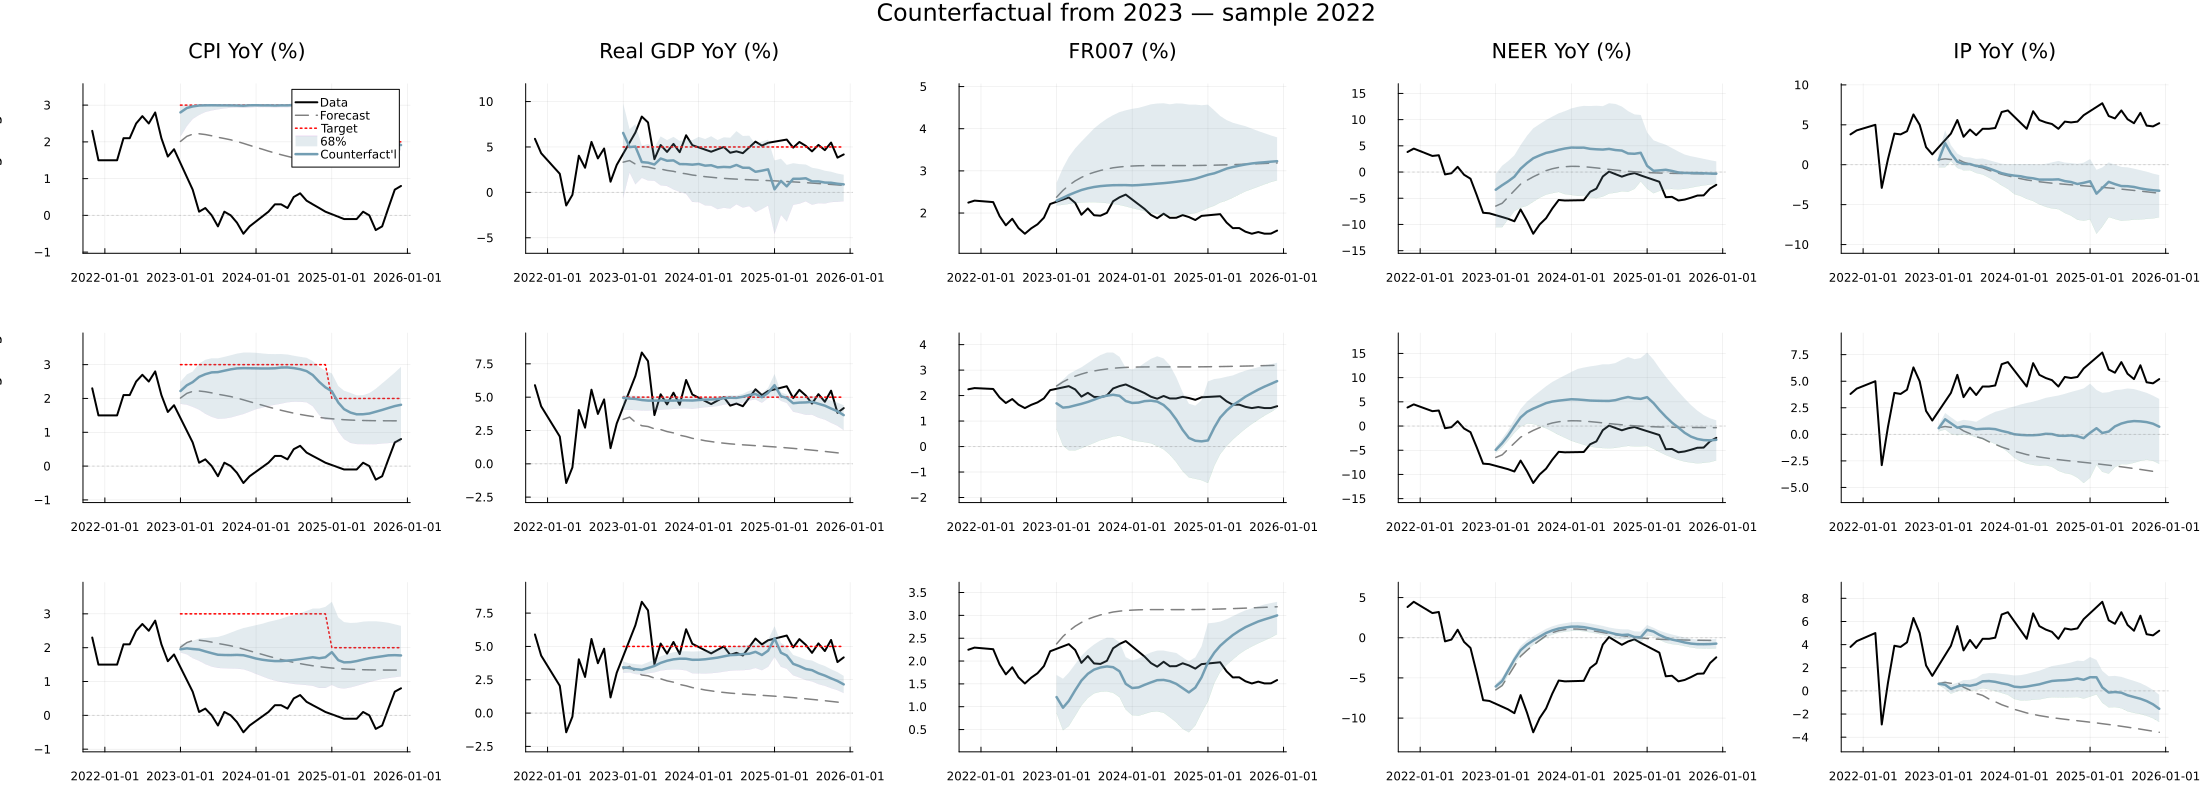
\includegraphics[width=1\textwidth,height=1.3\textheight,keepaspectratio]{outputs/main_results/2022/cnfctl_scenario_2023_s2022.png}\\
\scriptsize\textcolor{spgray}{\textit{ Counterfactual paths using data until 2022}}
\end{center}


\end{frame}
 
\begin{frame}{Headline Results}

\begin{center}
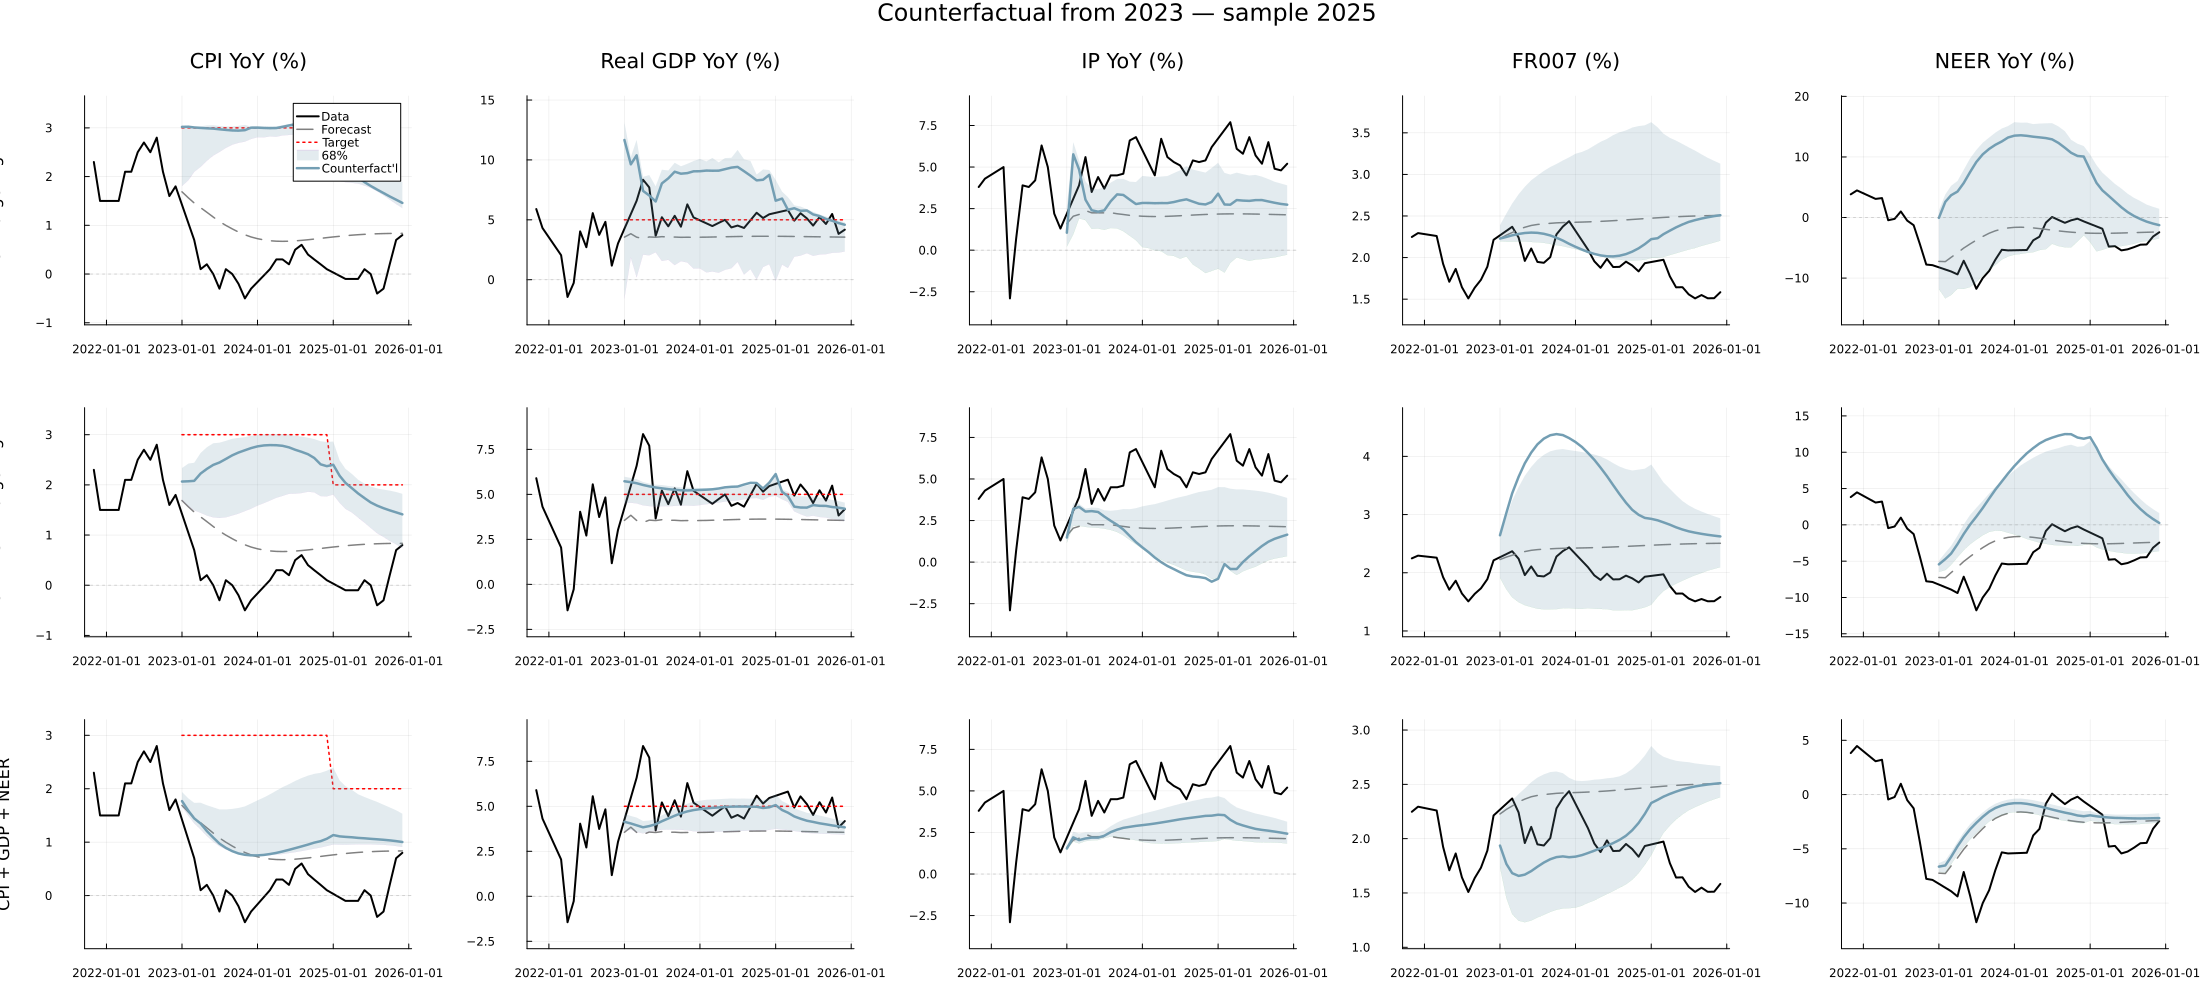
\includegraphics[width=1\textwidth,height=1.3\textheight,keepaspectratio]{outputs/main_results/2025/cnfctl_scenario_2023_s2025.png}\\
\scriptsize\textcolor{spgray}{\textit{ Counterfactual paths using data until 2025}}
\end{center}


\end{frame}

% ═══════════════════════════════════════════════════════════════════════════
% APPENDIX
% ═══════════════════════════════════════════════════════════════════════════
\appendix
 
% --- Appendix slide: regime switch motivation -------------------------------
\begin{frame}{Appendix --- Asymmetric GDP Gap Specification}
\hypertarget{app:regime}{}
 
\textbf{Construction.} Define the threshold indicator
$\mathds{1}_t^{-} = \mathds{1}\{\text{gdp\_gap}_t < 1\}$, then split:
\[
\text{gap\_pos}_t = \text{gdp\_gap}_t \cdot (1 - \mathds{1}_t^{-}),
\qquad
\text{gap\_neg}_t = \text{gdp\_gap}_t \cdot \mathds{1}_t^{-}.
\]
 
\textbf{Motivation.} Following Chen, Ren \& Zha (2018), the PBoC's response
to growth is hypothesised to be \emph{asymmetric}: monetary policy reacts
more aggressively when realized GDP growth falls meaningfully below the
official Government Work Report target than when it merely fluctuates around it. MANR2026 further estimated this threshold at around 1pp, meanining that the PBoC tends to tolerate small overshoots. 
 

 
\hyperlink{slide:rr}{\beamerreturnbutton{back}}
\end{frame}
 
% --- Appendix slide: actual vs predicted FR007 + residuals ------------------
\begin{frame}{Appendix --- Policy Rule Fit and Residuals}
\hypertarget{app:rrfit}{}
 
\textbf{Left} Actual FR007 vs.\ predicted FR007 from the rule regression.
\textbf{Right.} Estimated residual series $\widehat{\varepsilon}^{\text{MP}}_t$,
used as the narrative monetary policy shock.
 
\vspace{0.5em}
\begin{center}
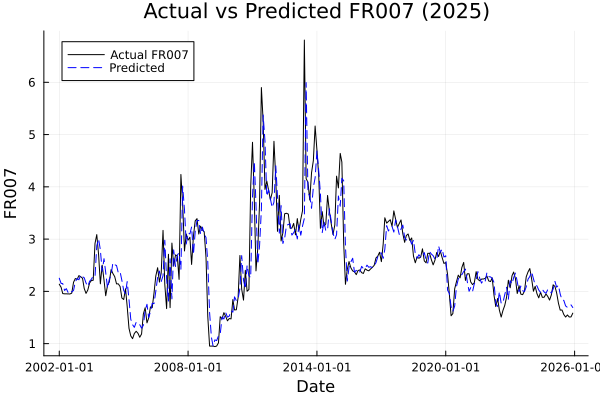
\includegraphics[width=0.48\textwidth,height=0.5\textheight,keepaspectratio]{outputs/robustness/2025/FR007_fit_comparison.png}
\hfill
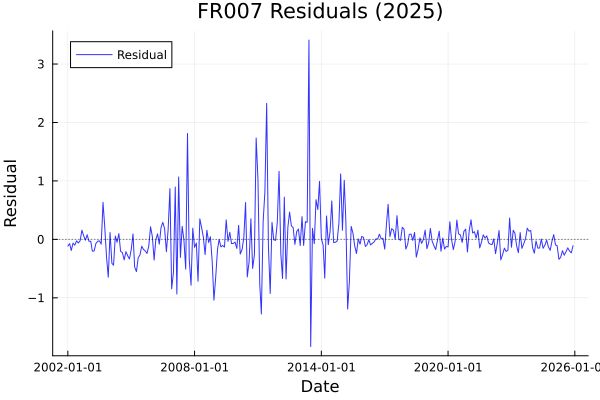
\includegraphics[width=0.48\textwidth,height=0.5\textheight,keepaspectratio]{outputs/robustness/2025/FR007_residuals_comparison.png}
\end{center}

\hyperlink{slide:rr}{\beamerreturnbutton{back}}
\end{frame}
 
% --- Appendix slide: monthly GDP construction (placeholder, will fill later) -
\begin{frame}{Appendix --- Monthly GDP Construction}
\hypertarget{app:gdp}{}
 
\textit{[To be filled in: Stock \& Watson (2010) distribution method,
adapted to NBS quarterly GDP (\begin{CJK}{UTF8}{gbsn}当季值\end{CJK}) using
the sum identity $Q_T = q_{3T-2} + q_{3T-1} + q_{3T}$, with monthly
indicators consumption / FAI / government spending / trade balance.]}

\begin{center}
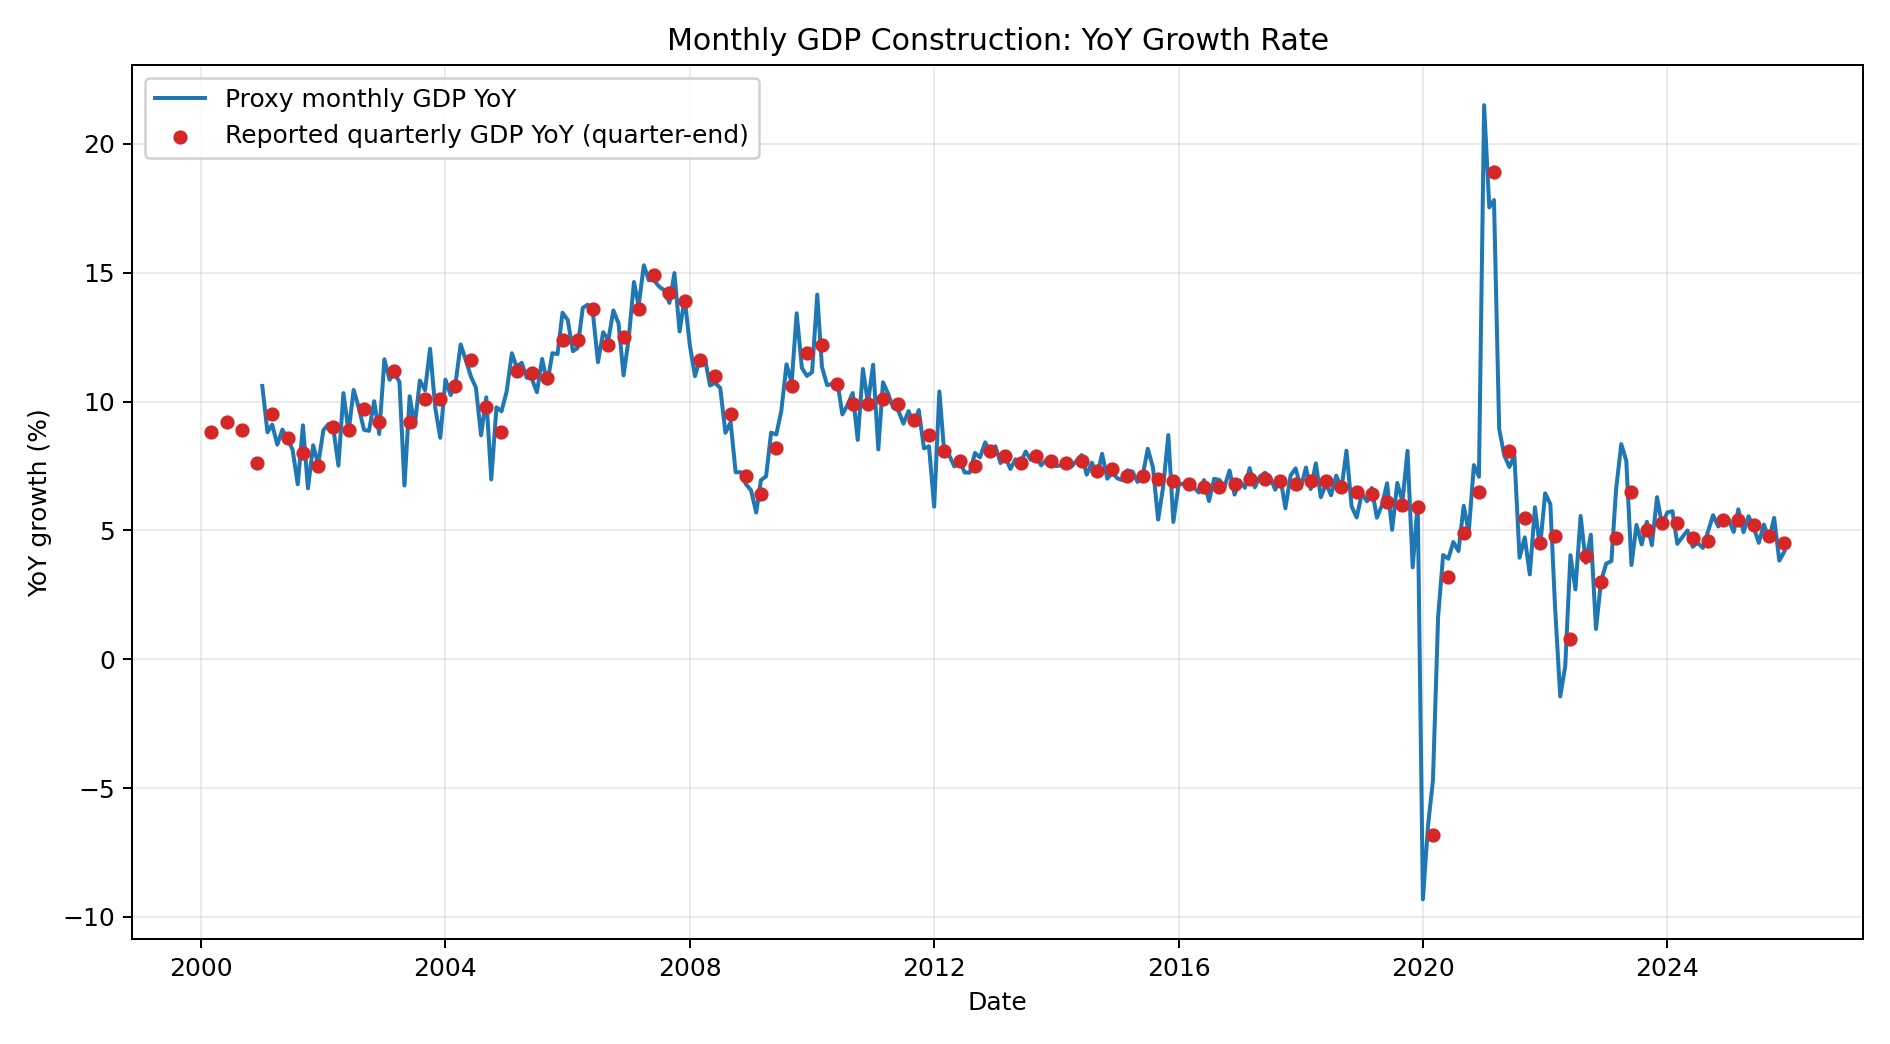
\includegraphics[width=0.9\textwidth,height=0.7\textheight,keepaspectratio]{outputs/diagnostics/gdp_quarterly_vs_proxy_monthly.png}
\end{center}
 
\hyperlink{slide:rr}{\beamerreturnbutton{back}}
\end{frame}

% --- Appendix slide: estimated monthly GDP vs. reported GDP ---------------
\begin{frame}{Appendix --- Forecast vs. Actual (Proxy) Monthly GDP}
\hypertarget{app:gdp_compare}{}



\begin{center}
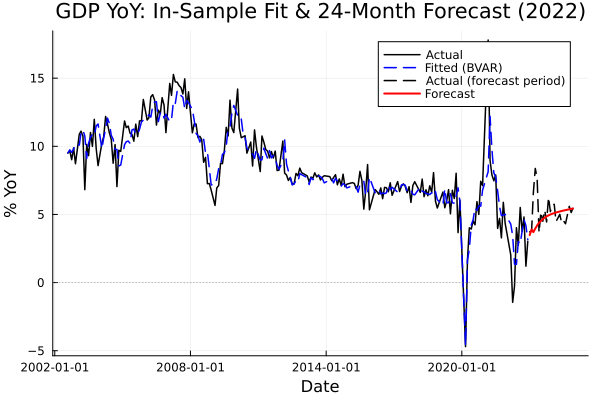
\includegraphics[width=0.9\textwidth,height=0.8\textheight,keepaspectratio]{outputs/diagnostics/2022/bvar_gdp_forecast.png}
\end{center}


\hyperlink{slide:ltp2}{\beamerreturnbutton{back}}
\end{frame}

% --- Appendix slide: narrative IRFs ----------------------------------------
\begin{frame}{Appendix --- Narrative Shock IRFs}
\hypertarget{app:narr_irf}{}

\begin{center}
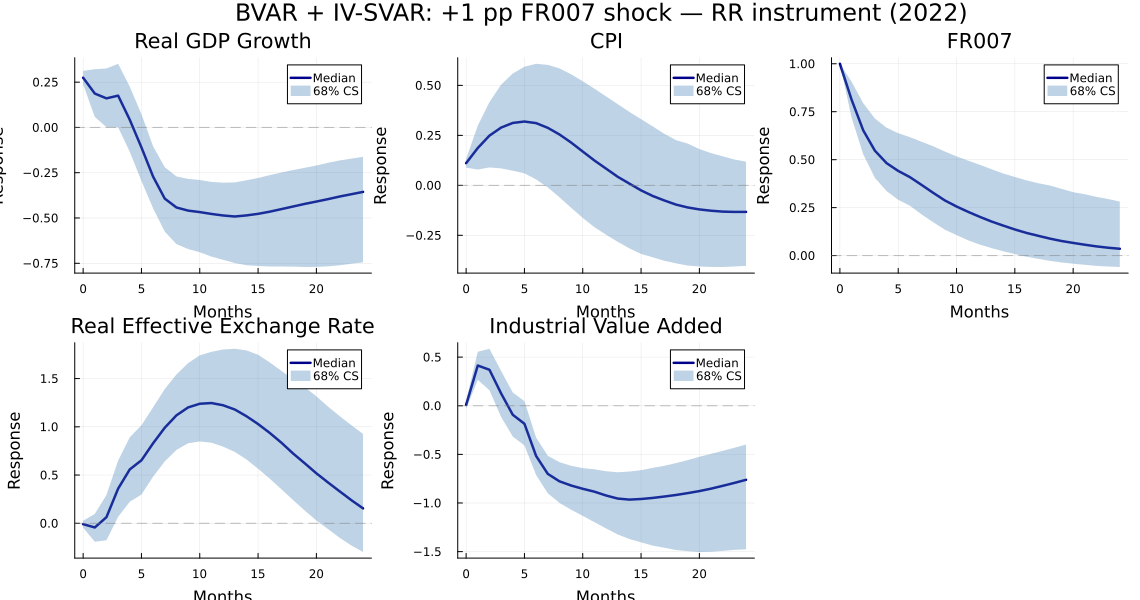
\includegraphics[width=0.92\textwidth,height=0.68\textheight,keepaspectratio]{outputs/main_results/2022/irf_bvar_iv_svar.png}
\end{center}

\scriptsize Initial increases in CPI mirrors the results from MANR2026, which they attribute to the fact that Chinese CPI takes into account the mortgage payments as housing costs, and thus can rise in response to a monetary tightening very quickly.

\hyperlink{slide:rr2}{\beamerreturnbutton{back}}
\end{frame}

% --- Appendix slide: HFI comparison (any announcement vs. rate-change-only) --
% --- Appendix slide: HFI IRFs ----------------------------------------------
\begin{frame}{Appendix --- HFI Shock IRFs}
\hypertarget{app:hfi_irf}{}

\begin{center}
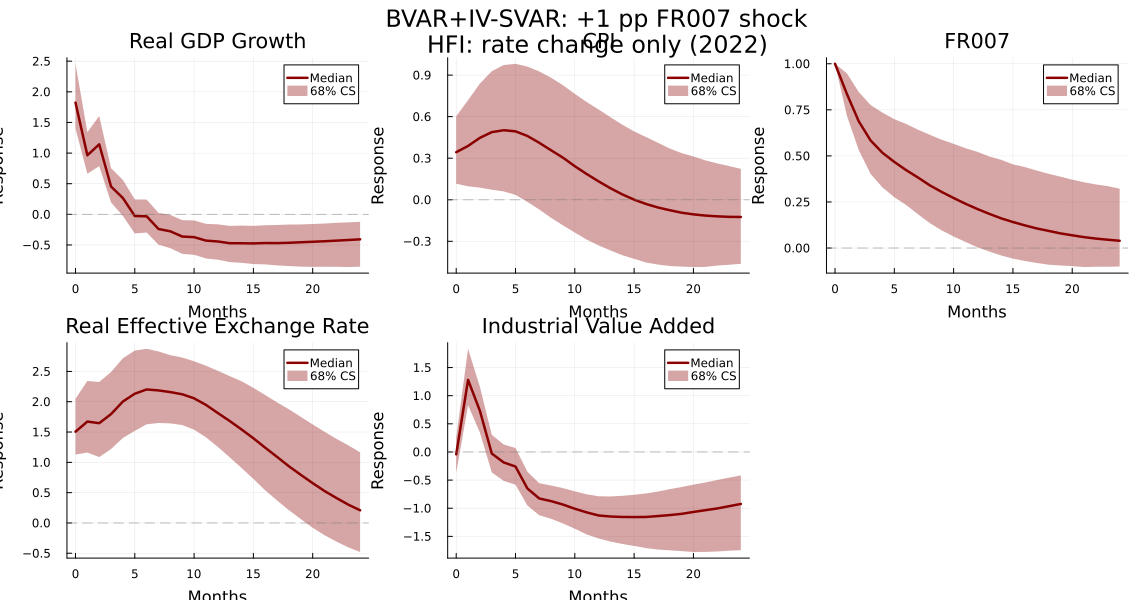
\includegraphics[width=0.92\textwidth,height=0.68\textheight,keepaspectratio]{outputs/main_results/2022/irf_hfi_shock_policy_change.png}
\end{center}


\hyperlink{slide:hfi}{\beamerreturnbutton{back}}
\end{frame}

% --- Appendix slide: HFI comparison (any announcement vs. rate-change-only) --
\begin{frame}{Appendix --- HFI Shocks: IRF Comparison}
\hypertarget{app:hfi_compare}{}

\textbf{Left.} IRF of Chinese economy to monetary policy shocks identified from FR007 surprises on \emph{any} PBoC policy announcement day.
\textbf{Right.} IRF using \emph{rate-change-only} identification --- cleaner shock, smaller sample size.

\vspace{0.5em}
\begin{center}
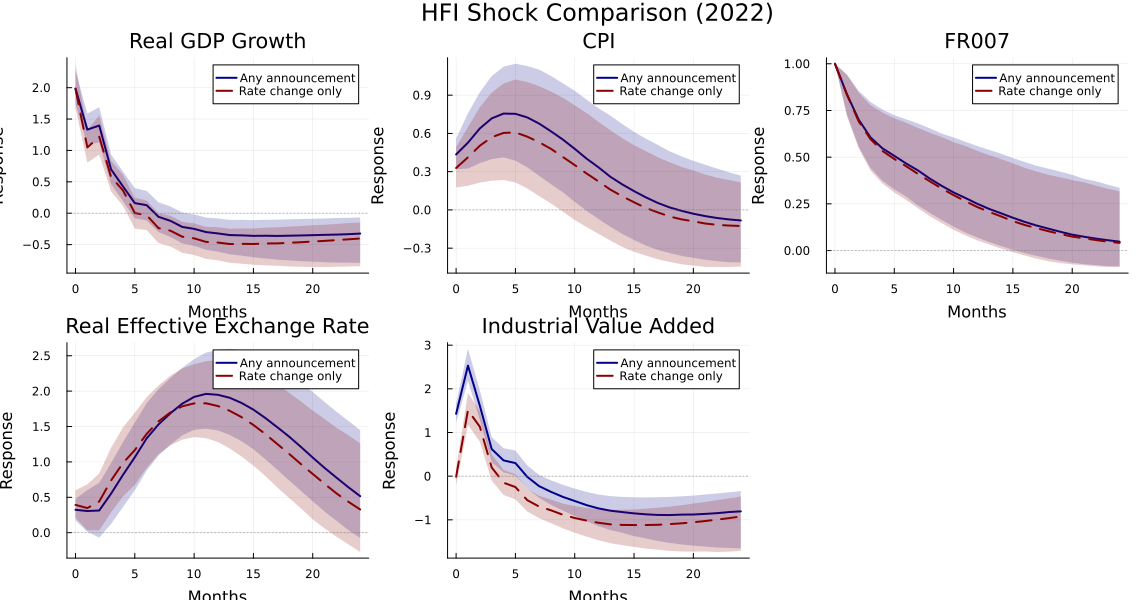
\includegraphics[width=0.92\textwidth,height=0.5\textheight,keepaspectratio]{outputs/main_results/2022/irf_hfi_comparison.png}
\end{center}

\vspace{0.3em}
\textcolor{spgray}{\scriptsize The rate-change-only series serves as the primary instrument in the counterfactual analysis, with the any-announcement series used for robustness checks.}

\hyperlink{slide:hfi}{\beamerreturnbutton{back}}
\end{frame}

% --- Appendix slide: HFI shock series --------------------------------------
\begin{frame}{Appendix --- HFI Monthly Shock Series}
\hypertarget{app:hfi_series}{}

\textbf{Monthly aggregation.} Daily FR007 surprises are summed within each calendar month, yielding the two monthly HFI shock series used in the counterfactual analysis.

\vspace{0.5em}
\begin{center}
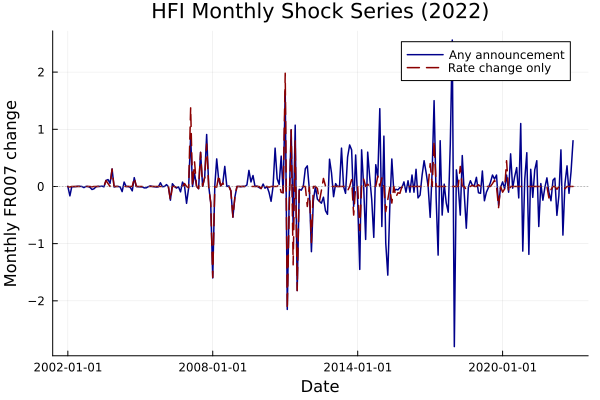
\includegraphics[width=0.92\textwidth,height=0.55\textheight,keepaspectratio]{outputs/main_results/2022/hfi_shock_series.png}
\end{center}

\vspace{0.3em}
\textcolor{spgray}{\scriptsize The solid line corresponds to shocks on any policy announcement day; the dashed line uses rate-change-only identification.}

\hyperlink{slide:hfi}{\beamerreturnbutton{back}}
\end{frame}

% --- Appendix slide: CMPI vs. FR007 comparison ---------------------------------
\begin{frame}{Appendix --- CMPI vs.\ FR007}
\hypertarget{app:cmpi_fr007}{}

\textbf{Specification choice.} Comparison of policy rule performance using FR007 (Composite Monetary Policy Indicator \textcolor{spgray}{\scriptsize our hybrid approach}) versus CMPI (Miranda-Agrippino, Nenova \& Rey 2026 baseline).

\vspace{0.5em}
\begin{center}
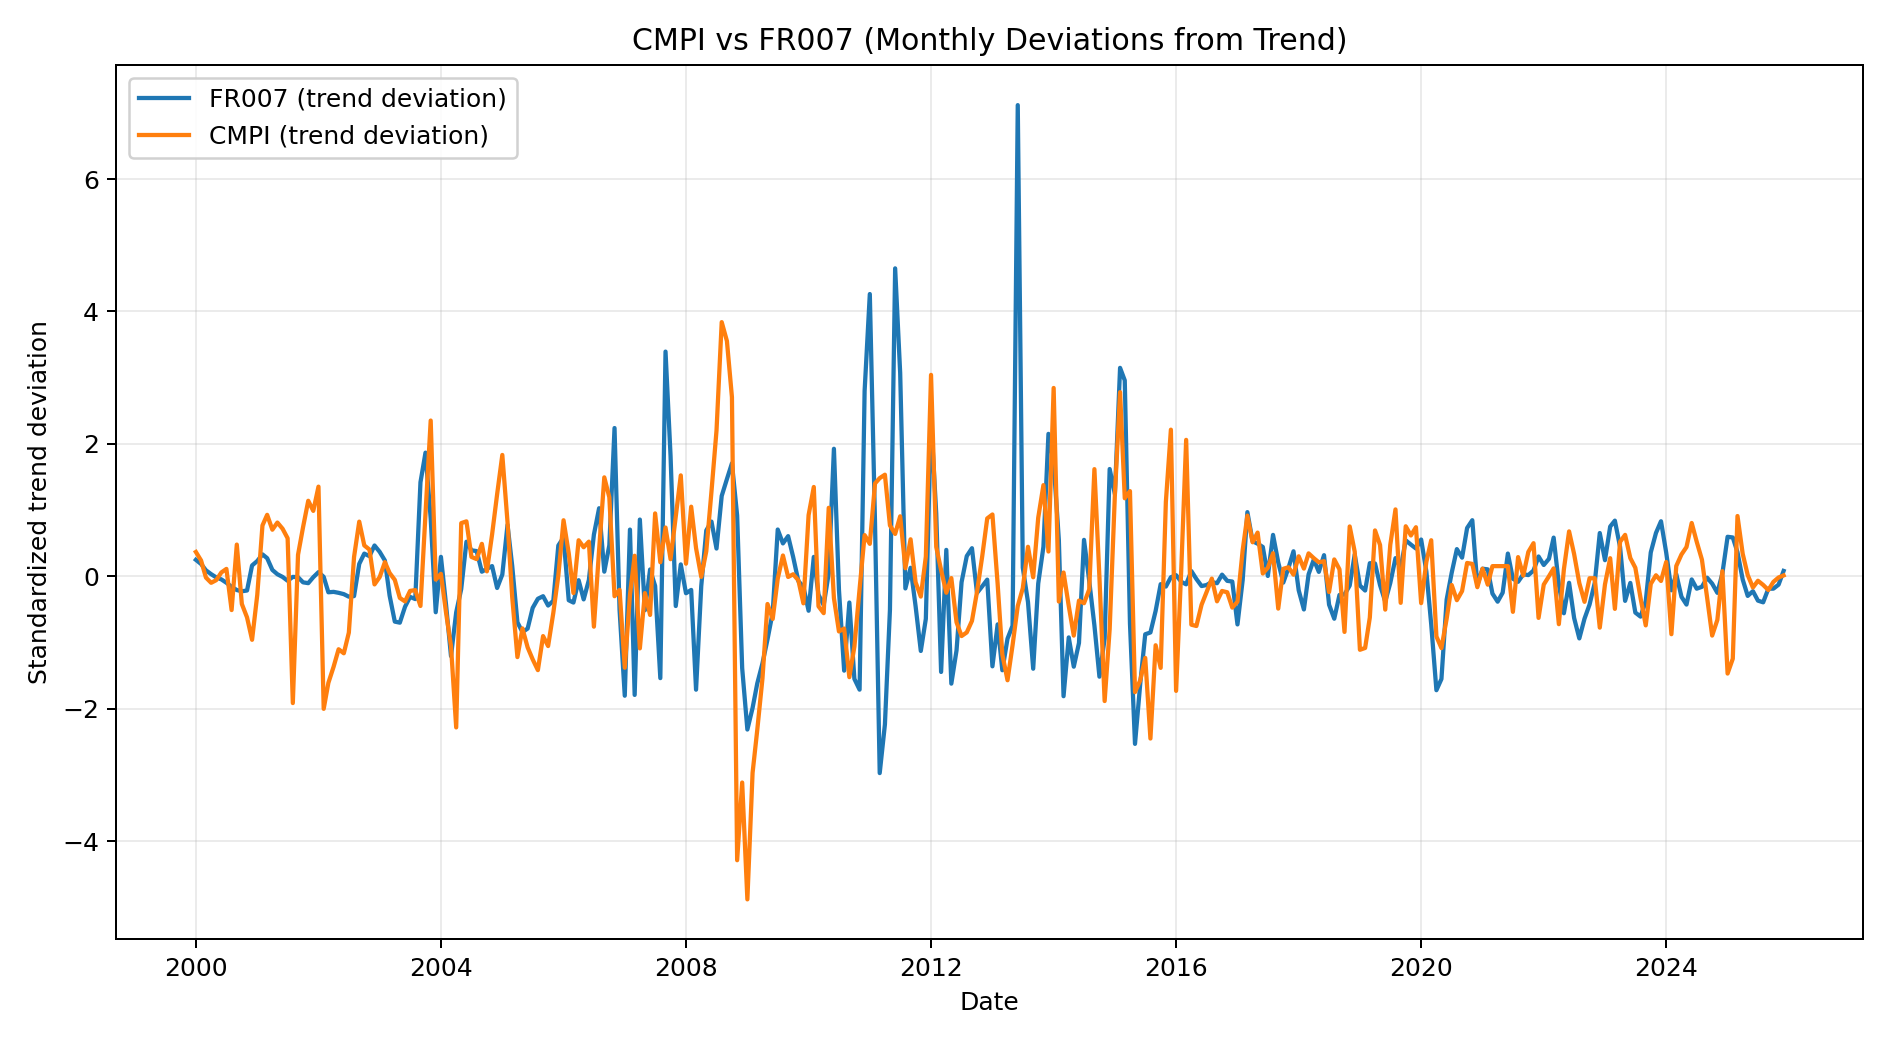
\includegraphics[width=0.9\textwidth,height=0.43\textheight,keepaspectratio]{outputs/robustness/cmpi_vs_fr007.png}
\end{center}

\vspace{0.3em}
\textcolor{spgray}{\scriptsize The choice to retain FR007 as the dependent variable while adopting MANR2026's FX specification ensures consistency with the high-frequency identification strategy, which relies on FR007 surprises on policy event dates.}

\hyperlink{slide:rr2}{\beamerreturnbutton{back}}
\end{frame}

\end{document}